\documentclass{article}
\usepackage[utf8]{inputenc}
\usepackage{array}
\usepackage{graphicx}
\title{Informe de la Tarea Investigativa II, presentado por los
estudiantes del equipo No. 30}
\author{Francisco Vicente Suárez Bellón C-212 \\
  Max Bengochea C-211}
\date{December 2022}

\begin{document}

\maketitle
\section*{Título: PERIODIC SOLUTIONS FOR SMALL AND LARGE DELAYS IN
A TUMOR-IMMUNE SYSTEM MODEL}
\subsection*{\centering Autores del articulo:\\
                 RADOUANE YAFIA
             }
\subsection*{\centering Revista: \\ 
                Electronic Journal of Differential Equations
             }
\subsection*{\centering Año: \\ 
                2006
             }
\subsection*{\centering Impacto: 1.282 }


\section{Valoración del artículo}
  \subsection*{Breve explicación}
  \noindent
   En el artículo a analizado el autor investiga mediante un modelo matemático el comportamiento 
   de un tumor y la respuesta del sistema inmune del individuo. La explicación científica-medica
   no es un argumento a analizar en dicho paper dado que no es su objetivo de estudio aunque si
   deja referenciado en que otros estudios y publicaciones se basa dicho modelo
   \subsection*{Problemática que se propone resolver
   }
   El artículo explica que el modelo matemático estudiado de otra publicación y su modificación 
   tiene una coincidencia lógica con los comportamientos biológicos del individuo, así como la no existencia
   de soluciones negativas o los puntos de estabilidad del mismo 
   \subsection*{Breve introducción}
   El modelo matemático que refleja la situación esta constituido por
    un sistema de 2 ecuaciones diferenciales (2.1) , donde “w”
     describe la respuesta inmune ante la aparición del tumor y “t” refleja 
     el tiempo que demora el sistema inmune en proporcionar una respuesta a 
    
\section{Introducción al problema a analizar}
\noindent En este articulo se hace referencia a un modelo de tumor inmune que expresa su comportamiento mediante 
 ecuaciones diferenciales en este se centran principalmente en su análisis de estabilidad y su estudio de
    soluciones periódicas. Para ello se hace uso de la teoría de la estabilidad de Lyapunov.
     El sistema el cual analizan en 
    profundidad es un sistema de ecuaciones diferenciales no ordinarias las cuales se 
    salen del objeto de este trabajo las cuales son:
    \centering
    \subsection*{Ecuaciones no ordinarias}
      $\frac{d x}{d t} $ =$\sigma + \omega x(t- \tau )y(t- \tau )-
        \delta x
        $
        \\
        $\frac{d y}{d t}$=$\alpha y(1-\beta y)-xy$



Sin embargo también nos proporcionan otro sistema de ecuaciones diferenciales ordinarias las
 cuales son el objeto de estudio 
en este trabajo 
\centering
   \subsection*{Sistema a trabajar}
        $\frac{d x}{d t} $ =$\sigma + \omega xy-
            \delta x
            $
            \\
            $\frac{d y}{d t}$=$\alpha y(1-\beta y)-xy$
      \\(2.1)
\section{Metodología}
\noindent 
  Para poder analizar este sistema no lineal de ecuaciones diferenciales ordinarias usaremos los 
  recursos numéricos como Runge-Kutta 4 y el método de Euler Modificado además
   de utilizar recursos computacionales para ilustrar los resultados obtenidos mediante
  gráficas.
  
  Comenzamos buscando los posibles puntos de equilibrio de este sistema de ecuaciones diferenciales ordinarias
  para ello buscamos para que valores ambas ecuaciones se hacen cero simultáneamente luego para obtener su
   análisis de estabilidad
  usaremos el teorema de Hartman–Grobman\\
  Para aplicar las hipótesis del teorema antes descrito es necesario "linealizar" el sistema dado que este no 
  es lineal por lo que se hace uso de la siguiente matriz de jacobiano del sistema respecto a  $x$ y $y$ respectivamente
 \subsection*{Matriz de jacobiano}
    \[
    \left(
    \begin{array}{lc}
      y\omega-\delta & x\omega\\
      -y & -x-y\alpha\beta+\alpha(-y\beta+1)
    \end{array}
    \right)
    \]
      
  \centering  
  
  Nos centraremos en el análisis en el punto de equilibrio $(0,0)$ dado que en dicho punto la matriz
   se convierte en una
  matriz diagonal lo cual facilita mucho el análisis de estabilidad de este punto de equilibrio.
  \subsection*{Matriz jacobina en (0,0)}
    \[
    \left(
    \begin{array}{lc}
      -\delta & 0\\
      0 & \alpha
    \end{array}
    \right)
    \]

  \noindent
    \subsection*{Análisis de estabilidad: \\ TEOREMA 2 Estabilidad de sistemas casi lineales}
      
      Sean $\lambda1$ y $\lambda2$ los eigenvalues de la matriz de
       coeficientes del sistema lineal dado 
      asociado con el sistema casi lineal. Entonces:\\
      1. Si  $\lambda1$ $=$ $\lambda2$ son eigenvalues reales e iguales, por consiguiente el punto crítico 
      (0, 0)  es un nodo o un punto espiral, y es asintóticamente estable si $\lambda1$
      $=$  $\lambda2$ $<$ 0, e inestable si $\lambda1$ $=$  $\lambda2$ $>$ 0.\\
      2. Si $\lambda1$ y $\lambda2$  son imaginarios puros, entonces (0, 0) es un centro o un punto espiral, 
      y puede ser asintóticamente estable, estable o inestable.\\

      3. En caso contrario —esto es, que  $\lambda1$ y  $\lambda2$ no sean reales e iguales o imaginarios 
      puros—, el punto crítico (0, 0) del sistema casi lineal  es del mismo 
      tipo y con la misma estabilidad que el punto crítico (0, 0) del sistema lineal 
      asociado

      %punto a=-1 d=1
    \section{Resultados}
       El tipo de estabilidad del punto (0,0) dependerá de los valores de: $\delta$ y $\alpha$
       \subsection{$\delta$=1 y $\alpha$=-1} 
         La matriz del jacobiano $:$
         \[
          \left(
          \begin{array}{lc}
            -1 & 0\\
            0 & -1
          \end{array}
          \right)
          \]         
          Con lo que es un nodo o punto espiral y asintóticamente estable 
          \subsection*{Planos Fase del punto }
          \noindent
          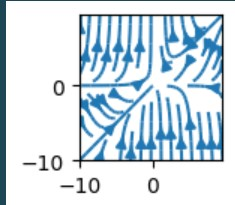
\includegraphics{Isoclinas de a=-1 y d=1.jpg}
           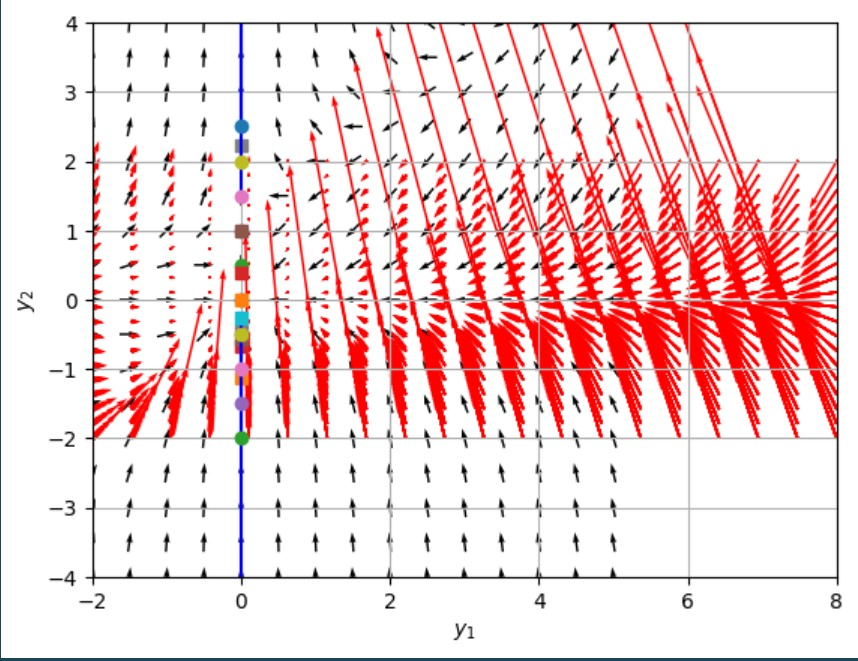
\includegraphics{Campo Vectoraal para a=-1 y d=1.jpg}\\
           
           %Punto a=1 d=-1
      \subsection*{$\delta$=-1 y $\alpha$=1}
        El tipo de estabilidad del punto (0,0) dependerá de los valores de: $\delta$ y $\alpha$
        La matriz del jacobiano quedaría
        \[
         \left(
         \begin{array}{lc}
           1 & 0\\
           0 & 1
         \end{array}
         \right)
         \]         
         Con lo que es un nodo o punto espiral y asintóticamente inestable
         \subsection*{Planos Fase del punto }
         \noindent
         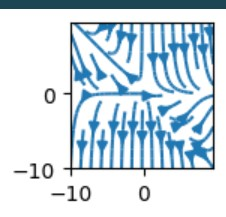
\includegraphics{isoclinas 2jpg.jpg}
          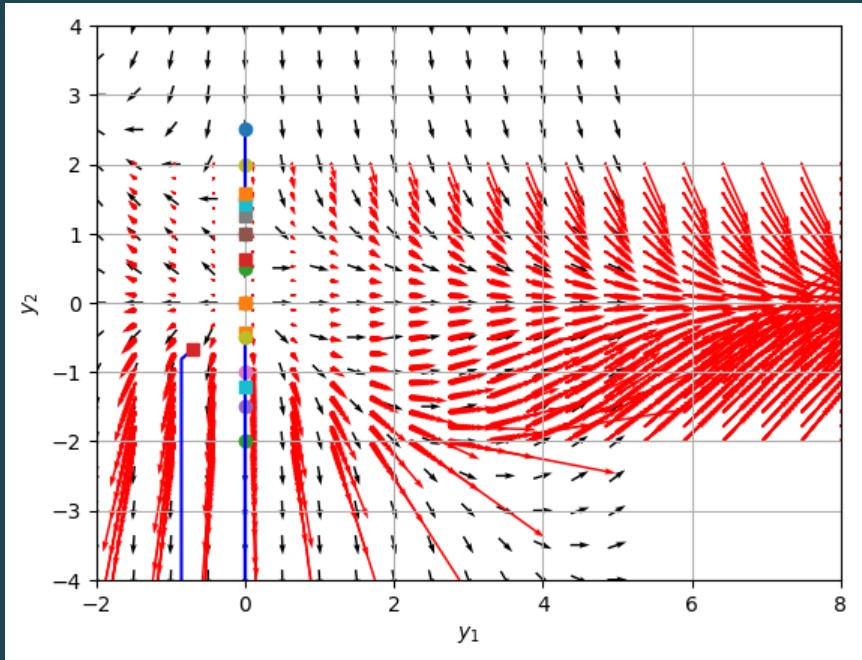
\includegraphics{Campo vectorail de d=-1 a1 .jpg}
        
          %Punto a=-2 d=1
      \subsection*{$\delta$=1 y $\alpha$=-2}
       
        La matriz del jacobiano quedaría
        \[
         \left(
         \begin{array}{lc}
           -1 & 0\\
           0 & -2
         \end{array}
         \right)
         \]         
         Con lo que es un nodo impropio estable
         \subsection*{Planos Fase del punto }
         \noindent
         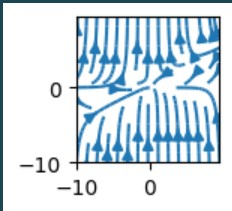
\includegraphics{isoclinas d=1 a=-2.jpg}
          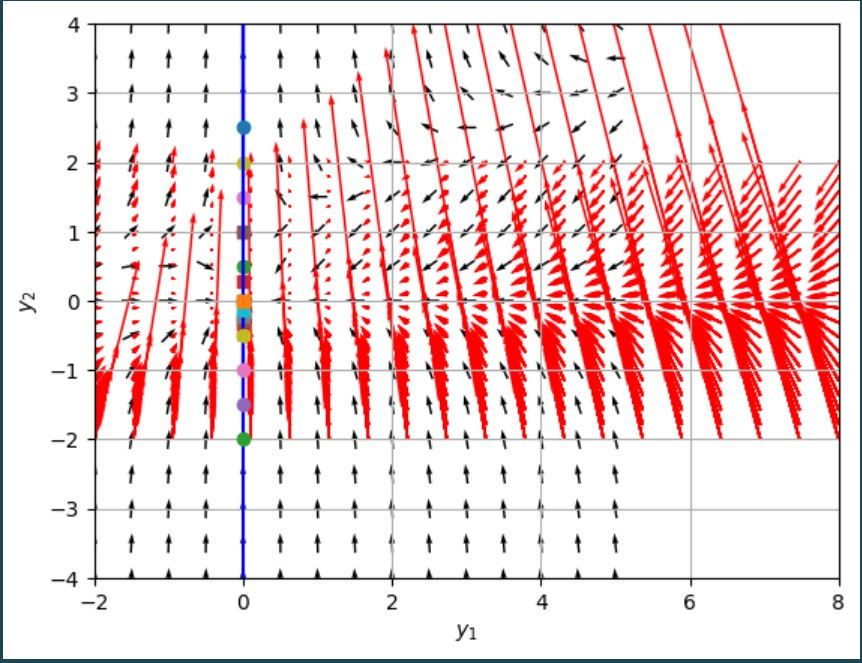
\includegraphics{Diagrama de fases para a-2 d1.jpg}


           %Punto a=1 d=1
     \subsection*{$\delta$=1 y $\alpha$=1}
       
        La matriz del jacobiano quedaría
        \[
         \left(
         \begin{array}{lc}
           -1 & 0\\
           0 & 1
         \end{array}
         \right)
         \]         
         Punto silla inestable
         \subsection*{Planos Fase del punto }
         \noindent
         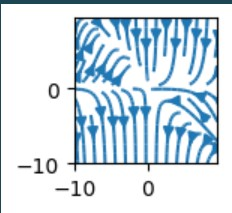
\includegraphics{punto silla inestable isoclinas.jpg}
          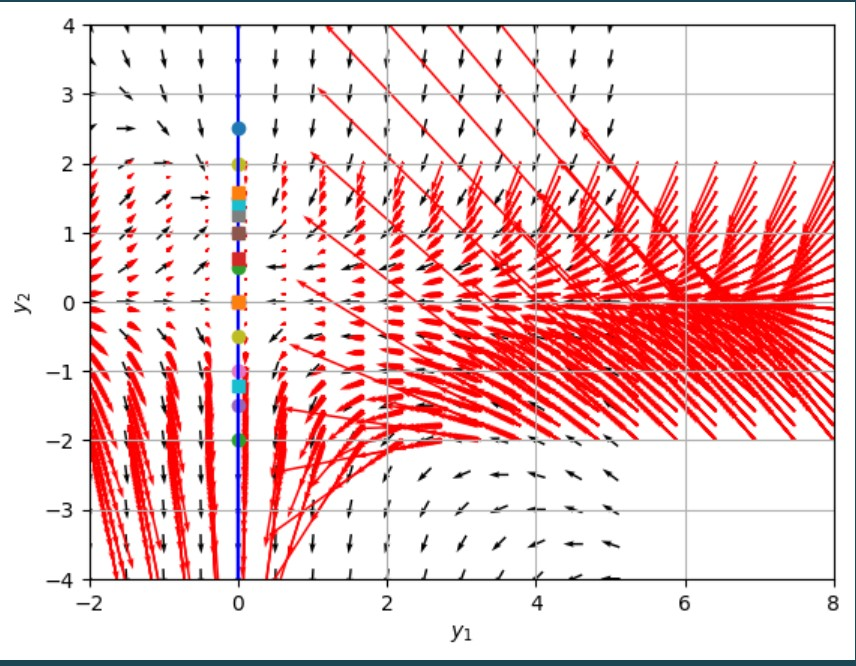
\includegraphics{punto silla inestable.jpg}
           
         %punto a=1 y d=-2
   \subsection*{$\delta$=1 y $\alpha$=1}
       
        La matriz del jacobiano quedaría
        \[
         \left(
         \begin{array}{lc}
           2 & 0\\
           0 & 1
         \end{array}
         \right)
         \]         
         Nodo impropio inestable
         \subsection*{Planos Fase del punto }
       \noindent
         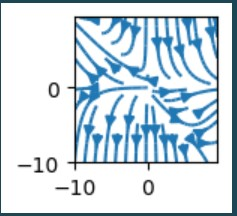
\includegraphics{isoclinas d=-2 a=1.jpg}
          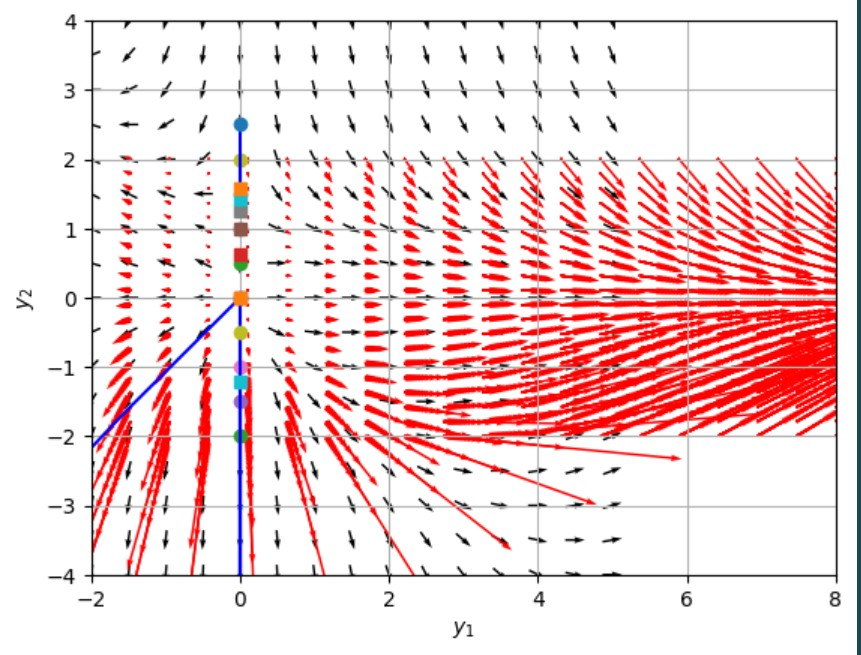
\includegraphics{vecotrial d=-2 a=1.jpg}

      \subsection*{Valores dados por métodos numéricos}
         Se mostrarán los resultados numéricos del sistema con valores $y=2x$
         con $x=100$ un tamaño de paso $h=1$ iniciado en $0$ y finalizado en $10$.
         Se compararan datos tanto de Runge-Kutta como de Euler Mejorado
           \subsection*{Runge-Kutta}
              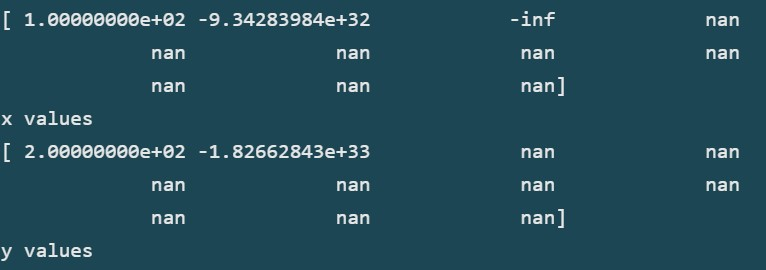
\includegraphics{valores de runge kutta para x=100 y y=200jpg.jpg}
            \\Gráficas:\\  
               Con respecto a al tiempo:           
            <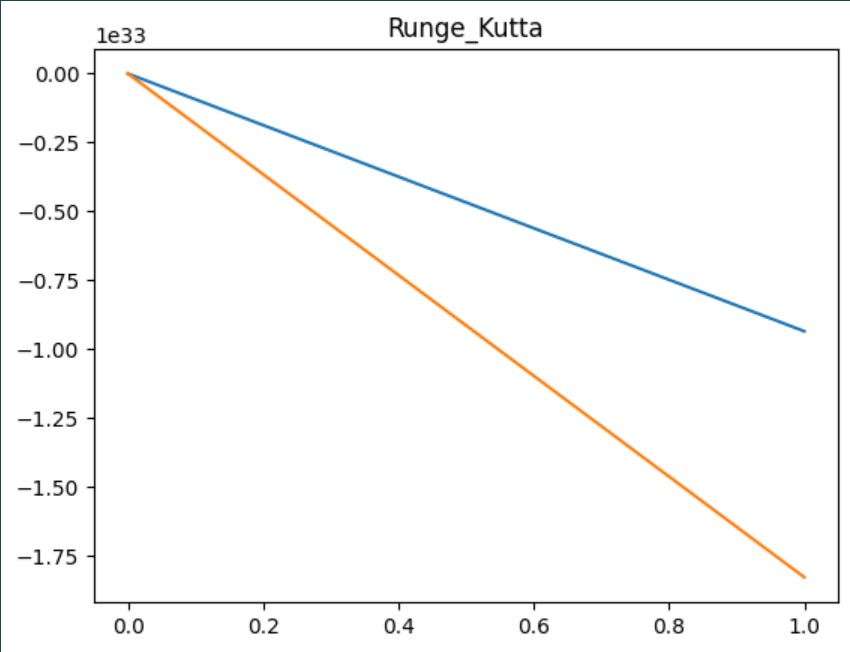
\includegraphics{Grafica runge_kutta.jpg}
               Con las funciones una respecto a la otra:
               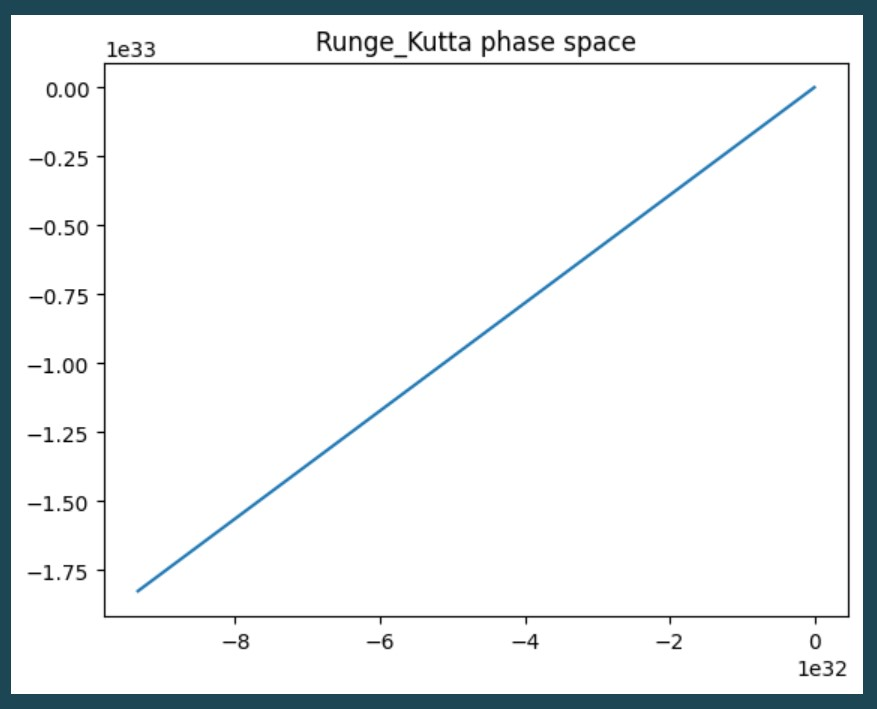
\includegraphics{x_y_rungekutta.jpg}
          \subsection*{Euler Mejorado}
             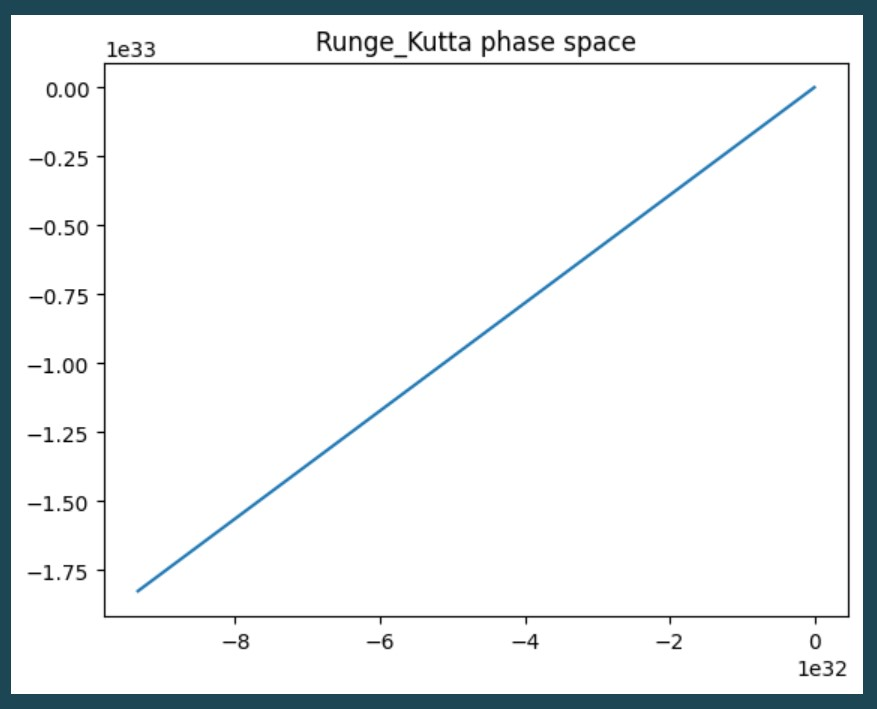
\includegraphics{x_y_values_euler.jpg}
             \\Gráficas:\\  
             Con respecto a al tiempo:
              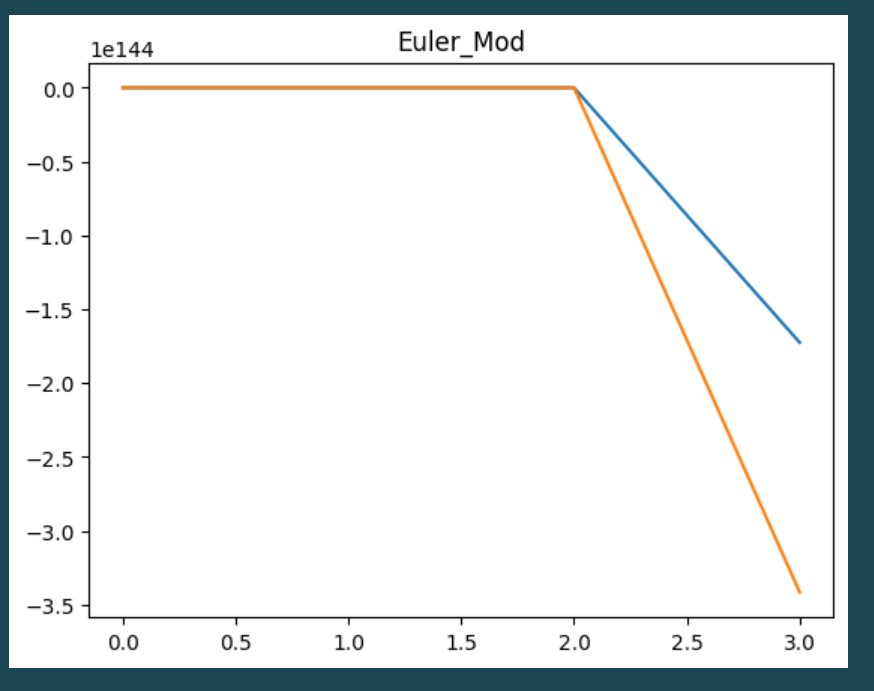
\includegraphics{eulermod.jpg}
             Con las funciones una respecto a la otra:
               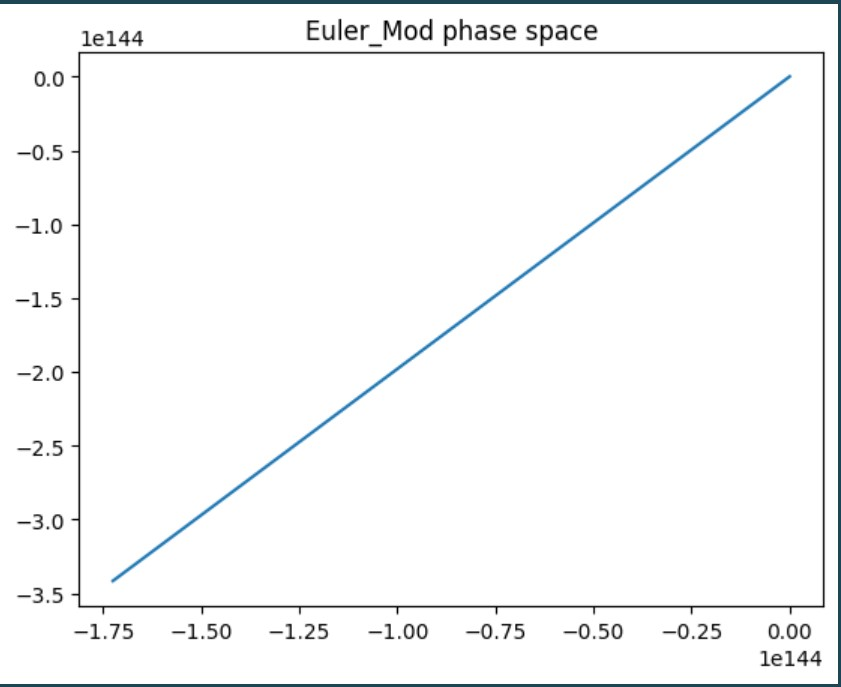
\includegraphics{eulermodx,y.jpg}
          \subsection*{Plano Fase}
            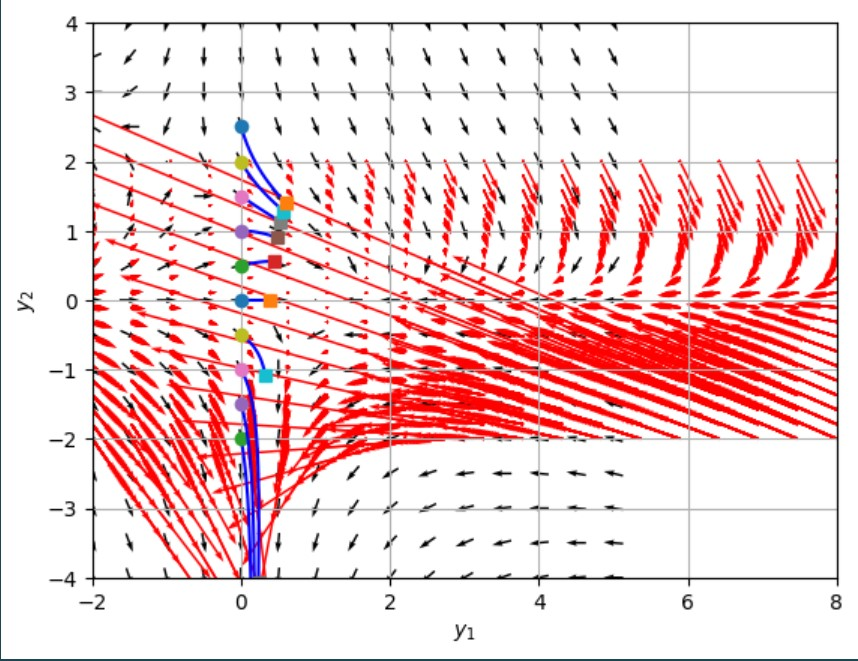
\includegraphics{planofasenumericccc.jpg}
             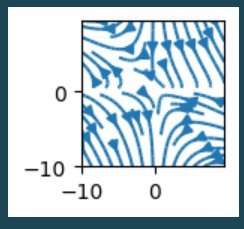
\includegraphics{isoclinas numerico.jpg}
          \subsection*{Análisis}
             En los resultados anteriores se evidencia que para números de esa magnitud las soluciones 
             son más grandes que la aritmética de la computadora y además se ve que dado la naturaleza de los
             métodos numéricos Euler Mejorado nos permite aunque perdiendo precisión tener otro dato más

     


\end{document}

  
